%
% Qucs Test Report: SPICE to Qucs conversion: Test File 3
%
% Copyright (C) 2007 Mike Brinson <mbrin72043@yahoo.co.uk>
%
% Permission is granted to copy, distribute and/or modify this document
% under the terms of the GNU Free Documentation License, Version 1.1
% or any later version published by the Free Software Foundation.
%

% redefine subfigure caption
\renewcommand{\thesubfigure}{\thefigure(\alph{subfigure})}
\makeatletter
  \renewcommand{\@thesubfigure}{\thesubfigure:\space}
  \renewcommand{\p@subfigure}{}
\makeatother

% redefine subtable caption
\renewcommand{\thesubtable}{\thetable(\alph{subtable})}
\makeatletter
  \renewcommand{\@thesubtable}{\thesubtable:\space}
  \renewcommand{\p@subtable}{}
\makeatother

\tutsection{Introduction}
\tutsubsection{Title}
SPICE 2g6 and 3f5 resistors.

\tutsubsection{SPICE specification}

\begin{flushleft}
Format: SPICE 2g6\footnote{See section 6.1, SPICE 2g6 user's guide.}: \hspace*{5mm}
\textbf{RX N+ N- value [ TC=TC1 [,TC2] ]}                                                                                                                                                                            \end{flushleft}

Notes: 
\begin{enumerate}
 \item Characters [ and ] enclose optional items 
 \item Resistors begin with letter R.
 \item X denotes name of resistor.
 \item N+ and N- are the positive and negative nodes respectively.
 \item Equations:
\begin{flushleft}
$ TNOM = $ Nominal temperature; default 27\degree C.
\linebreak 
  $\Delta T = T-TNOM
\linebreak 
  R(T) = R(TNOM)+\left[ 1+TC1 \cdot \Delta T+TC2 \cdot \Delta T^{2} \right] $
\end{flushleft}
\end{enumerate}

\begin{flushleft}
Format: SPICE 3f5\footnote{See sections 3.1.1 and 3.1.2, SPICE 3f6 user's guide.}:
\begin{enumerate}
\item Standard resistors: \textbf{RX N+ N- value}
\item Semiconductor resistors: 

\textbf{RX N+ N- [value] [mname] [L=length] [W=width] [TEMP=T]}                                                                                                                                                                                                                            \end{enumerate}
 \end{flushleft}

\begin{flushleft}
Notes: 
  \begin{enumerate}
   \item Characters [ and ] enclose optional items 
 \item Resistors begin with letter R.
 \item X denotes name of resistors.
 \item N+ and N- are the positive and negative nodes respectively.
 \item mname; if specified the resistance is calculated from the process information given in entry .model mname.
 \item L is the length of the resistor.
 \item W is the width of the resistor.
 \item mname .model type R  parameters:
 \begin{itemize}
\item TC1  : First order temperature coefficient; default 0.0.$\Omega / \degree C$.
\item TC2  : Second order temperature coefficient; default 0.0. $\Omega / \degree C^{2}$.
\item RSH  : Sheet resistance; default -. $\Omega$ per square.
\item DEFW : Default width; default 1e-6m.
\item NARROW : Narrowing due to side etching; default 0.0m.
\item TNOM : Nominal temperature; default 27 $\degree C$.
\end{itemize}

 
  \item Equations
   $R = RSH \cdot \dfrac{L-NARROW}{W-NARROW}$


   $R(T) = R(TNOM)+\left[ 1+TC1 \cdot \Delta T+TC2 \cdot \Delta T^{2} \right] $

Where $\Delta T = T-T_{0}$: T is the circuit temperature and $T_{0}$ the nominal temperature. 
  \end{enumerate}

\end{flushleft}


\tutsection{Test code and schematic}
\begin{flushleft}

SPICE code: File \verb|S2Q_test3_a.cir|

\end{flushleft}

\begin{lstlisting}[
 language=Clean, 
 basicstyle=\small]

* SPICE to Qucs syntax test file 
* SPICE 2g6 resistors.
*
.subckt S2Q_test3_a p01 p02 p03
v1 1 0 DC 1v
r1 1 p01 10k
r2 p01 0 10k
*
v2 2 0 dc 1v
r3 2 p02  10k tc=0.01
r4 p02 0  10k
*
v3 3 0 Dc 1v
r5 3 p03  10k tc=0.01 0.015
r6 p03 0 10k
.ends
.end


\end{lstlisting}

\newpage 
\begin{flushleft}

SPICE code: File \verb|S2Q_test3_b.cir|

\end{flushleft}

\begin{lstlisting}[
 language=Clean, 
 basicstyle=\small]

* SPICE to Qucs syntax test file 
* SPICE 3f5 resistors.
*
.subckt S2Q_test3_a p01 p02 p03
v1 1 0 DC 1v
r1 1 p01 10k
r2 p01 0 10k
*
v2 2 0 dc 1v
r3 2 p02  RMOD1 L=10u W=1u
r4 p02 0  10k
.model RMOD1 R(RSH=50 DEFW=2e-6 NARROW=1e-7)
*
.ends
.end
\end{lstlisting}


\begin{flushleft}
 

\end{flushleft}

\begin{figure}
  \centering
  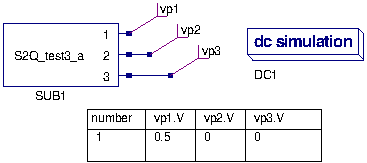
\includegraphics[width=0.8\linewidth]{S2Q_test3_a_sch}
  \caption{March 13: SPICE to Qucs conversion: Test3 schematic plus output table for SPICE 2g6 test1: linear resistors}
  \label{fig:S2Qtest3_1}
\end{figure} 
 
\begin{flushleft}

\newpage 
\tutsection{History of simulation results}
\tutsubsection{March 13 2007, Simulation tests by Mike Brinson}

A: SPICE 2g6 tests:



\textbf{Test 1} [v2, r3, v3, and r5 commented]: Linear resistors: Vp1: PASS correct output voltage.


\textbf{Test 2} [v3, and r5  commented]: SPICE 2g6 resistor with first order temperature coefficient:\textbf{ FAIL} - inncorrect Qucs netlist.


Qucs netlist line 14: checker error, extraneous property `TC' is invalid in `R:R3'


 
\end{flushleft}


Qucs netlist:
\begin{lstlisting}[
 language=Clean, 
 basicstyle=\small]
# Qucs 0.0.11  /media/hda2/S2Q_test3_prj/S2Q(test3_a).sch

.Def:S2Q_test3_a _net0 _net1 _net2
Sub:X1 _net0 _net1 _net2 gnd Type="S2Q_test3_a_cir"
.Def:End

.Def:S2Q_test3_a_cir _netP01 _netP02 _netP03 _ref
  .Def:S2Q_TEST3_A _ref _netP01 _netP02 _netP03
  Vdc:V1 _net1 _ref U="1V"
  R:R1 _net1 _netP01 R="10k"
  R:R2 _netP01 _ref R="10k"
  Vdc:V2 _net2 _ref U="1V"
  R:R3 _net2 _netP02 R="10k" TC="0.01"
  R:R4 _netP02 _ref R="10k"
  R:R6 _netP03 _ref R="10k"
  .Def:End
  Sub:X1 _ref _netP01 _netP02 _netP03 Type="S2Q_TEST3_A"
.Def:End


Sub:SUB1 vp1 vp2 vp3 Type="S2Q_test3_a"
.DC:DC1 Temp="26.85" reltol="0.001" abstol="1 pA" vntol="1 uV"
 saveOPs="no" MaxIter="150" saveAll="no" convHelper="none" Solver="CroutLU"
\end{lstlisting}

\begin{flushleft}

\textbf{Test 3} [v2, r2, and r3 commented]: \textbf{FAIL} - netlist not passed correctly.

Qucs error message: line 14: syntax error, unexpected Floats, expecting Eol.

\end{flushleft}

Qucs netlist:
\begin{lstlisting}[
 language=Clean, 
 basicstyle=\small]
# Qucs 0.0.11  /media/hda2/S2Q_test3_prj/S2Q(test3_a).sch

.Def:S2Q_test3_a _net0 _net1 _net2
Sub:X1 _net0 _net1 _net2 gnd Type="S2Q_test3_a_cir"
.Def:End

.Def:S2Q_test3_a_cir _netP01 _netP02 _netP03 _ref
.Def:End


Sub:SUB1 vp1 vp2 vp3 Type="S2Q_test3_a"
.DC:DC1 Temp="26.85" reltol="0.001" abstol="1 pA" 
vntol="1 uV" saveOPs="no" MaxIter="150" saveAll="no"
convHelper="none" Solver="CroutLU"

\end{lstlisting}


\begin{flushleft}
B: SPICE 3f5 tests

\textbf{Test1}: SPICE file \verb|S2Q_test3_b.cir| fails to convert to Qucs netlist format, giving the following error message:

line10 : syntax error, unexpected identifier, expecting Digits or Floats.

SPICE 3f5 Semiconductor resistors not implemented?
\end{flushleft}

\tutsubsection{March 15 2007, Simulation tests by Mike Brinson}


\begin{flushleft}

Qucs CVS code modifications:   
\begin{flushleft}
\begin{itemize}
 \item  * \verb|scan_spice.l|: Lexer modifications for the Spice 2g6 resistor
        syntax were necessary. Stefan Jahn
 \item   *\verb| parse_spice.y|: Allow Spice 2g6 syntax for resistors, also
        fixed netlist grammar for Spice 3f5 models. Stefan Jahn
 \item  * \verb|check_spice.cpp|: Handle R semiconductor model correctly as
        well as the Spice 2g6 syntax for the temperature coefficients. Stefan Jahn

\end{itemize}             \end{flushleft}

SPICE code: File \verb|S2Q_test3_a.cir|

\begin{itemize}
 \item Vp01.V: \textbf{PASS}; correct dc output.
 \item Vp02.V: \textbf{PASS}; correct dc output for TEMP=TNOM.
 \item Vp03.V: \textbf{PASS}; correct dc output for TEMP=TNOM.
 \end{itemize}

\begin{flushleft}
 NOTES:
\begin{itemize}
 \item The Vp02 and Vp03 test results are only correct for TEMP=TNOM.
 \item SPICE 2g6 simulates circuit performance at temperature set by the value of TNOM; 27 \degree C by default.
 \item Circuits can be simulated at other temperatures by using a .TEMP control statement; which has the format


 .TEMP   T1 [ T2 [ T3 ..... ] ]


 Unfortunately the Qucsconv program does not recognise this statement so there appears to be no way of changing the temperature of SPICE 2g6 resistors that have TC1 and TC2 temperature coefficients in their netlist entries.
\item Adding SPICE 2g6 statement .TEMP 50 to file \verb|S2Q_test3_a.cir| gives the following error:

spice notice, no .END directive found, continuing 
line 18: syntax error, unexpected Identifier, expecting \verb|$end| 
\end{itemize}

\end{flushleft}

\begin{flushleft}
Qucs netlist:
\begin{lstlisting}[
 language=Clean, 
 basicstyle=\small]
# Qucs 0.0.11  /media/hda2/S2Q_test3_prj/S2Q(test3_a).sch

.Def:S2Q_test3_a _net0 _net1 _net2
Sub:X1 _net0 _net1 _net2 gnd Type="S2Q_test3_a_cir"
.Def:End

.Def:S2Q_test3_a_cir _netP01 _netP02 _netP03 _ref
  .Def:S2Q_TEST3_A _ref _netP01 _netP02 _netP03
  Vdc:V1 _net1 _ref U="1V"
  R:R1 _net1 _netP01 R="10k"
  R:R2 _netP01 _ref R="10k"
  Vdc:V2 _net2 _ref U="1V"
  R:R3 _net2 _netP02 R="10k" Tc1="0.01"
  R:R4 _netP02 _ref R="10k"
  Vdc:V3 _net3 _ref U="1V"
  R:R5 _net3 _netP03 R="10k" Tc1="0.01" Tc2="0.015"
  R:R6 _netP03 _ref R="10k"
  .Def:End
  Sub:X1 _ref _netP01 _netP02 _netP03 Type="S2Q_TEST3_A"
.Def:End


.DC:DC1 Temp="50" reltol="0.001" abstol="1 pA" vntol="1 uV"
 saveOPs="no" MaxIter="150" saveAll="no" convHelper="none"
 Solver="CroutLU"
Sub:SUB1 vp1 vp2 vp3 Type="S2Q_test3_a"

\end{lstlisting}

\begin{figure}
  \centering
  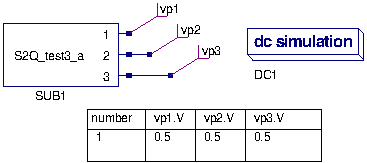
\includegraphics[width=0.8\linewidth]{S2Q_test3_a2}
  \caption{March 15: SPICE to Qucs conversion: SPICE 2g6 resistor schematic plus output table }
  \label{fig:S2Qtest3_2}
\end{figure} 

\newpage 
SPICE code: File \verb|S2Q_test3_b.cir|

\begin{itemize}
 \item Vp01.V: \textbf{PASS}; correct dc output.
 \item Vp02.V: \textbf{PASS}; correct dc output.
 
 \end{itemize}

Qucs netlist:
\begin{lstlisting}[
 language=Clean, 
 basicstyle=\small]
# Qucs 0.0.11  /media/hda2/S2Q_test3_prj/S2Q(test3_b).sch

.Def:S2Q_test3_b _net0 _net1
Sub:X1 _net0 _net1 gnd Type="S2Q_test3_b_cir"
.Def:End

.Def:S2Q_test3_b_cir _netP01 _netP02 _ref
  .Def:S2Q_TEST3_A _ref _netP01 _netP02
  Vdc:V1 _net1 _ref U="1V"
  R:R1 _net1 _netP01 R="10k"
  R:R2 _netP01 _ref R="10k"
  Vdc:V2 _net2 _ref U="1V"
  R:R3 _net2 _netP02 R="550"
  R:R4 _netP02 _ref R="10k"
  .Def:End
  Sub:X1 _ref _netP01 _netP02 Type="S2Q_TEST3_A"
.Def:End


Sub:SUB1 vp01 vp02 Type="S2Q_test3_b"
.DC:DC1 Temp="26.85" reltol="0.001" abstol="1 pA" vntol="1 uV"
 saveOPs="no" MaxIter="150" saveAll="no" convHelper="none" Solver="CroutLU"

\end{lstlisting}
\end{flushleft}



SPICE code: File \verb|S2Q_test3_c.cir|
\begin{lstlisting}[
 language=Clean, 
 basicstyle=\small]
* SPICE to Qucs syntax test file 
* SPICE 3f5 resistors : Temperature effects.
*
.subckt S2Q_test3_a p01 p02 p03 p04 p05 p06 p07 p08 p09 p10
v1 1 0 DC 1v
r1 1 p01 10k
r2 p01 0 10k
*
v2 2 0 dc 1v
r3 2 p02  10k  RMOD1 
r4 p02 0  10k
.model RMOD1 R(TC1=0.01 TC2=0.015)
*
v3 3 0 dc 1v
r5 3 p03   10k RMOD1 TEMP=30
r6 p03 0  10k
*
v4 4 0 dc 1v
r7 4 p04   10k RMOD1 TEMP=40
r8 p04 0  10k
*
v5 5 0 dc 1v
r9 5 p05   10k RMOD1 TEMP=50
r10 p05 0  10k
*
v6 6 0 dc 1v
r11 6 p06   10k RMOD1 TEMP=60
r12 p06 0  10k
*
v7 7 0 dc 1v
r13 7 p07   10k RMOD1 TEMP=70
r14 p07 0  10k
*
v8 8 0 dc 1v
r15 8 p08   10k RMOD1 TEMP=80
r16 p08 0  10k
*
v9 9 0 dc 1v
r17 9 p09   10k RMOD1 TEMP=90
r18 p09 0  10k
*
v10 10 0 dc 1v
r19 10 p10   10k RMOD1 TEMP=100
r20 p10  0  10k
.ends
.end

\end{lstlisting}
\end{flushleft}

\begin{flushleft}

\begin{itemize}
 \item Vp01.V: \textbf{PASS}; correct dc output.
 \item Vp02.V: \textbf{PASS}; correct dc output.
 \item Vp03.V: \textbf{PASS}; correct dc output.
 \item Vp04.V: \textbf{PASS}; correct dc output.
 \item Vp05.V: \textbf{PASS}; correct dc output.
 \item Vp06.V: \textbf{PASS}; correct dc output.
 \item Vp07.V: \textbf{PASS}; correct dc output.
 \item Vp08.V: \textbf{PASS}; correct dc output.
 \item Vp09.V: \textbf{PASS}; correct dc output.
 \item Vp20.V: \textbf{PASS}; correct dc output. 
\end{itemize}

NOTES: \begin{itemize}
\item In SPICE 3f5 TEMP values attached to resistors override the global value of TEMP.                                                     
\item SPICE 3f5 differs from SPICE 2g6 in that it does not allow the control statement .TEMP.

                                  \end{itemize}

\end{flushleft}

\newpage 
\begin{figure}
  \centering
  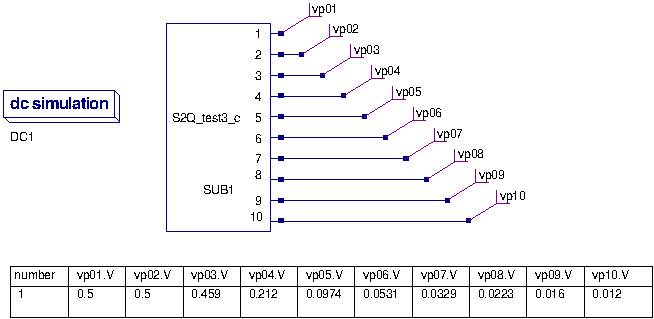
\includegraphics[width=0.8\linewidth]{S2Q_test3_c}
  \caption{March 15: SPICE to Qucs conversion: Test3 schematic plus output for SPICE 3f5 test c} 
  \label{fig:S2Qtest3_2}
\end{figure} 


Qucs netlist:
\begin{lstlisting}[
 language=Clean, 
 basicstyle=\small]
# Qucs 0.0.11  /media/hda2/S2Q_test3_prj/s2Q(test3_c).sch

.Def:S2Q_test3_c _net0 _net1 _net2 _net3 _net4 _net5 _net6 _net7 _net8 _net9
Sub:X1 _net0 _net1 _net2 _net3 _net4 _net5 _net6 _net7 _net8 _net9
 gnd Type="S2Q_test3_c_cir"
.Def:End

.Def:S2Q_test3_c_cir _netP01 _netP02 _netP03 _netP04 _netP05 
_netP06 _netP07 _netP08 _netP09 _netP10 _ref
  .Def:S2Q_TEST3_A _ref _netP01 _netP02 _netP03 _netP04 
_netP05 _netP06 _netP07 _netP08 _netP09 _netP10
  Vdc:V1 _net1 _ref U="1V"
  R:R1 _net1 _netP01 R="10k"
  R:R2 _netP01 _ref R="10k"
  Vdc:V2 _net2 _ref U="1V"
  R:R3 _net2 _netP02 R="10k" Tc1="0.01" Tc2="0.015"
  R:R4 _netP02 _ref R="10k"
  Vdc:V3 _net3 _ref U="1V"
  R:R5 _net3 _netP03 R="10k" Temp="30" Tc1="0.01" Tc2="0.015"
  R:R6 _netP03 _ref R="10k"
  Vdc:V4 _net4 _ref U="1V"
  R:R7 _net4 _netP04 R="10k" Temp="40" Tc1="0.01" Tc2="0.015"
  R:R8 _netP04 _ref R="10k"
  Vdc:V5 _net5 _ref U="1V"
  R:R9 _net5 _netP05 R="10k" Temp="50" Tc1="0.01" Tc2="0.015"
  R:R10 _netP05 _ref R="10k"
  Vdc:V6 _net6 _ref U="1V"
  R:R11 _net6 _netP06 R="10k" Temp="60" Tc1="0.01" Tc2="0.015"
  R:R12 _netP06 _ref R="10k"
  Vdc:V7 _net7 _ref U="1V"
  R:R13 _net7 _netP07 R="10k" Temp="70" Tc1="0.01" Tc2="0.015"
  R:R14 _netP07 _ref R="10k"
  Vdc:V8 _net8 _ref U="1V"
  R:R15 _net8 _netP08 R="10k" Temp="80" Tc1="0.01" Tc2="0.015"
  R:R16 _netP08 _ref R="10k"
  Vdc:V9 _net9 _ref U="1V"
  R:R17 _net9 _netP09 R="10k" Temp="90" Tc1="0.01" Tc2="0.015"
  R:R18 _netP09 _ref R="10k"
  Vdc:V10 _net10 _ref U="1V"
  R:R19 _net10 _netP10 R="10k" Temp="100" Tc1="0.01" Tc2="0.015"
  R:R20 _netP10 _ref R="10k"
  .Def:End 
  Sub:X1 _ref _netP01 _netP02 _netP03 _netP04 _netP05 _netP06 _netP07
 _netP08 _netP09 _netP10 Type="S2Q_TEST3_A"
.Def:End


Sub:SUB1 vp01 vp02 vp03 vp04 vp05 vp06 vp07 vp08 vp09 vp10 Type="S2Q_test3_c"
.DC:DC1 Temp="26.8" reltol="0.001" abstol="1 pA" vntol="1 uV" saveOPs="no" 
MaxIter="150" saveAll="no" convHelper="none" Solver="CroutLU"


\end{lstlisting}

\tutsubsection{March 18 2007, Simulation tests by Mike Brinson}

\begin{flushleft}
 More SPICE 3f5 Temperature tests.

SPICE code: File \verb|S2Q_test3_f.cir|
\begin{lstlisting}[
 language=Clean, 
 basicstyle=\small]
* SPICE to Qucs syntax test file 
* SPICE 3f5 resistors.
* Temperature tests.
*
.subckt S2Q_test3_f p01 p02 p03 p04 
v1 1 0 DC 1v
r1 1 p01 10k
r2 p01 0 10k
*
*
v2 2 0 dc 1v
r3 2 p02  10k  RMOD1 TEMP=50
r4 p02 0  10k
.model RMOD1 R(TC1=0.01 TC2=0.015)
*
v3 3 0 dc 1v
r5 3 p03  10k  RMOD1 
r6 p03 0  10k
.model RMOD1 R(TC1=0.01 TC2=0.015 TNOM=100)
*
v4 4 0 dc 1v
r7 4 p04  10k  RMOD1
r8 p04 0  10k
.model RMOD1 R(TC1=0.01 TC2=0.015)
*
.ends
.OPTION TNOM=40
.end
\end{lstlisting}
\end{flushleft}

\begin{flushleft}

\begin{itemize}
 \item Vp01.V: \textbf{PASS}; correct dc output.
 \item Vp02.V: \textbf{PASS}; correct dc output.
 \item Vp03.V: \textbf{FAIL}; dc output does not change with changes in .OPTION TEMP or TNOM.
 \item Vp04.V: \textbf{FAIL}; dc output does not change with changes in .OPTION TEMP or TNOM.
\end{itemize}

NOTES: \begin{itemize}
\item In SPICE 3f5 TEMP values attached to resistors override the global value of circuit temperature
\item Output Vp02 is correct the value of R3 being determined by TEMP=50, TC1=0.01 and TC2=0.015 during the resistance calculation. 
\item Using SPICE statements .OPTION TNOM=XX or .OPTION TEMP=XX appears to have no effect on resistance calculations.
\item Similarly, adding TNOM=XX to a R model appears not to affect the resistance calculations. 

                                  \end{itemize}

\end{flushleft}

\newpage 
\begin{figure}
  \centering
  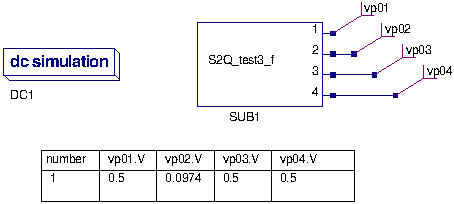
\includegraphics[width=0.8\linewidth]{S2Q_test3_f_sch}
  \caption{March 18: SPICE to Qucs conversion: Test3 schematic plus output for SPICE 3f5 test f} 
  \label{fig:S2Qtest3_3}
\end{figure} 


Qucs netlist:
\begin{lstlisting}[
 language=Clean, 
 basicstyle=\small]
# Qucs 0.0.11  /media/hda2/S2Q_test3_prj/S2Q(test3_f).sch

.Def:S2Q_test3_f _net0 _net1 _net2 _net3
Sub:X1 _net0 _net1 _net2 _net3 gnd Type="S2Q_test3_f_cir"
.Def:End

.Def:S2Q_test3_f_cir _netP01 _netP02 _netP03 _netP04 _ref
  .Def:S2Q_TEST3_F _ref _netP01 _netP02 _netP03 _netP04
  Vdc:V1 _net1 _ref U="1V"
  R:R1 _net1 _netP01 R="10k"
  R:R2 _netP01 _ref R="10k"
  Vdc:V2 _net2 _ref U="1V"
  R:R3 _net2 _netP02 R="10k" Temp="50" Tc1="0.01" Tc2="0.015"
  R:R4 _netP02 _ref R="10k"
  Vdc:V3 _net3 _ref U="1V"
  R:R5 _net3 _netP03 R="10k" Tc1="0.01" Tc2="0.015"
  R:R6 _netP03 _ref R="10k"
  Vdc:V4 _net4 _ref U="1V"
  R:R7 _net4 _netP04 R="10k" Tc1="0.01" Tc2="0.015"
  R:R8 _netP04 _ref R="10k"
  .Def:End
  Sub:X1 _ref _netP01 _netP02 _netP03 _netP04 Type="S2Q_TEST3_F"
.Def:End


Sub:SUB1 vp01 vp02 vp03 vp04 Type="S2Q_test3_f"
.DC:DC1 Temp="26.8" reltol="0.001" abstol="1 pA" vntol="1 uV" 
saveOPs="no" MaxIter="150" saveAll="no" convHelper="none" Solver="CroutLU"

\end{lstlisting}

\tutsection{March 25 2007, Simulation tests by Mike Brinson}
\begin{flushleft}
 Code modifications:

\begin{itemize}
 \item * \verb|scan_spice.l, parse_spice.y|: Accept .TEMP syntax (Spice 2g6)
        in lexer and parser. Stefan Jahn.
\end{itemize}

SPICE code: File \verb|S2Q_test3_a.cir|\linebreak SPICE statements .OPTION TNOM=50  and .TEMP 50 are now accepted in the SPICE to Qucs translation process. HOWEVER, at the moment (Qucs 0.0.12) global circuit temperature parameters are not implemented in the Qucs simulator and cannot be changed via these statements.

\end{flushleft}
\begin{flushleft}

SPICE code: File \verb|S2Q_test3_f.cir|\linebreak
SPICE code modification due to test bug caused by RMOD1 being referenced in each test.\linebreak
New code:
\begin{lstlisting}[
 language=Clean, 
 basicstyle=\small]
* SPICE to Qucs syntax test file 
* SPICE 3f5 resistors.
* Temperature tests.
*
.subckt S2Q_test3_f p01 p02 p03 p04 
v1 1 0 DC 1v
r1 1 p01 10k
r2 p01 0 10k
v2 2 0 dc 1v
r3 2 p02  10k  RMOD1 TEMP=50
r4 p02 0  10k
.model RMOD1 R(TC1=0.01 TC2=0.015)
v3 3 0 dc 1v
r5 3 p03  10k  RMOD2 
r6 p03 0  10k
.model RMOD2 R(TC1=0.01 TC2=0.015 TNOM=100)
v4 4 0 dc 1v
r7 4 p04  10k  RMOD3
r8 p04 0  10k
.model RMOD3 R(TC1=0.01 TC2=0.015)
.ends
.OPTION TNOM=40
.end
\end{lstlisting}

\end{flushleft}

\begin{figure}
  \centering
  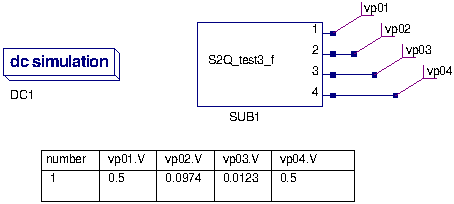
\includegraphics[width=0.8\linewidth]{S2Q_test3_f_2}
  \caption{March 25: SPICE to Qucs conversion: Test3 schematic plus output for SPICE 3f5 test f} 
  \label{fig:S2Qtest3_4}
\end{figure} 


\newpage 
Qucs netlist:
\begin{lstlisting}[
 language=Clean, 
 basicstyle=\small]
# Qucs 0.0.12  /media/hda2/S2Q_test3_prj/S2Q(test3_f).sch

.Def:S2Q_test3_f _net0 _net1 _net2 _net3
Sub:X1 _net0 _net1 _net2 _net3 gnd Type="S2Q_test3_f_cir"
.Def:End

.Def:S2Q_test3_f_cir _netP01 _netP02 _netP03 _netP04 _ref
  .Def:S2Q_TEST3_F _ref _netP01 _netP02 _netP03 _netP04
  Vdc:V1 _net1 _ref U="1V"
  R:R1 _net1 _netP01 R="10k"
  R:R2 _netP01 _ref R="10k"
  Vdc:V2 _net2 _ref U="1V"
  R:R3 _net2 _netP02 R="10k" Temp="50" Tc1="0.01" Tc2="0.015"
  R:R4 _netP02 _ref R="10k"
  Vdc:V3 _net3 _ref U="1V"
  R:R5 _net3 _netP03 R="10k" Tc1="0.01" Tc2="0.015" Tnom="100"
  R:R6 _netP03 _ref R="10k"
  Vdc:V4 _net4 _ref U="1V"
  R:R7 _net4 _netP04 R="10k" Tc1="0.01" Tc2="0.015"
  R:R8 _netP04 _ref R="10k"
  .Def:End
  Sub:X1 _ref _netP01 _netP02 _netP03 _netP04 Type="S2Q_TEST3_F"
.Def:End


Sub:SUB1 vp01 vp02 vp03 vp04 Type="S2Q_test3_f"
.DC:DC1 Temp="26.8" reltol="0.001" abstol="1 pA" vntol="1 uV" 
saveOPs="no" MaxIter="150" saveAll="no" convHelper="none" Solver="CroutLU"


\end{lstlisting}

\begin{flushleft}

\begin{itemize}
 \item Vp01.V: \textbf{PASS}; correct dc output.
 \item Vp02.V: \textbf{PASS}; correct dc output.
 \item Vp03.V: \textbf{PASS}; correct dc output.
 \item Vp04.V: \textbf{FAIL}; dc output does not change with changes in .OPTION TNOM = 40. The Qucs simulator does NOT implement a global temperature parameter but allocates separate temperatures to each component.
\end{itemize}
\vspace{5mm}
NOTES: \begin{itemize}
\item In SPICE 3f5 TEMP values attached to resistors override the global value of circuit temperature
\item Output Vp02 is correct, the value of R3 being determined by TEMP=50, TC1=0.01 and TC2=0.015. 
\item Output Vp03 is correct, the value of R5 being determined by TNOM=100, TC1=0.01 and TC2=0.015.
\item Output VP04 is 0.5 because .OPTION TNOM=40 has no effect on the temperature of resistor R8. By default the temperature of R8 is set to 26.85$\degree C$. 

                                  \end{itemize}

\end{flushleft}

\tutsection{References}
\begin{enumerate}
 \item A. Vladimirescu, Kaihe Zhang, A.R. Newton, D.O Pederson A. Sangiovanni-Vincentelli, SPICE 2G User's Guide (10 Aug 1981), Department of Electrical Engineering and Computer Sciences, University of California, Berkeley, Ca., 94720.
\item B. Johnson, T. Quarles, A.R. Newton, P.O. Pederson, A.Sangiovanni-Vincentelli, SPICE3 Version 3f User's Manual (October 1972),  Department of Electrical Engineering and Computer Sciences, University of California, Berkeley, Ca., 94720.
\item Andrei Vladimirescu, THE SPICE book,1994, John Wiley and Sons. Inc., ISBN 0-471-609-26-9.
\end{enumerate}


